\documentclass{standalone}
\usepackage{tikz}
\usetikzlibrary{patterns, positioning}

\begin{document}
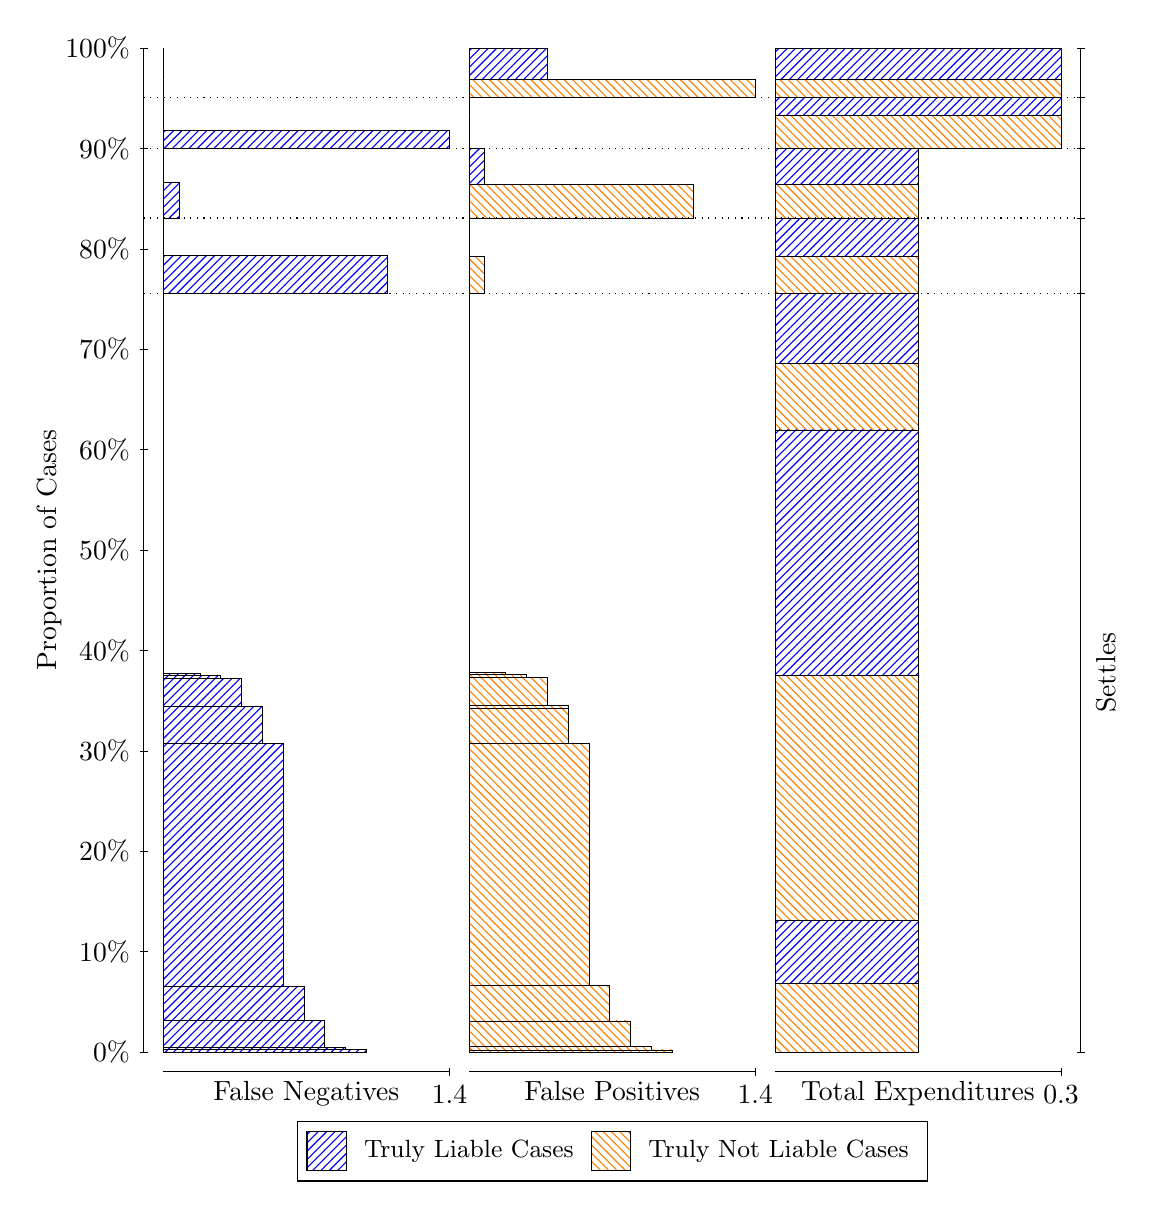
\begin{tikzpicture}
\draw[black, very thin] (1.5,1.75) -- (1.5,14.5);
\node[rotate=90, anchor=center] at (0.3, 8.125) {Proportion of Cases};
\draw[black, very thin] (1.45,1.75) -- (1.55,1.75);
\node[anchor=east] at (1.45, 1.75) {0\%};
\draw[black, very thin] (1.45,3.025) -- (1.55,3.025);
\node[anchor=east] at (1.45, 3.025) {10\%};
\draw[black, very thin] (1.45,4.3) -- (1.55,4.3);
\node[anchor=east] at (1.45, 4.3) {20\%};
\draw[black, very thin] (1.45,5.575) -- (1.55,5.575);
\node[anchor=east] at (1.45, 5.575) {30\%};
\draw[black, very thin] (1.45,6.85) -- (1.55,6.85);
\node[anchor=east] at (1.45, 6.85) {40\%};
\draw[black, very thin] (1.45,8.125) -- (1.55,8.125);
\node[anchor=east] at (1.45, 8.125) {50\%};
\draw[black, very thin] (1.45,9.4) -- (1.55,9.4);
\node[anchor=east] at (1.45, 9.4) {60\%};
\draw[black, very thin] (1.45,10.675) -- (1.55,10.675);
\node[anchor=east] at (1.45, 10.675) {70\%};
\draw[black, very thin] (1.45,11.95) -- (1.55,11.95);
\node[anchor=east] at (1.45, 11.95) {80\%};
\draw[black, very thin] (1.45,13.225) -- (1.55,13.225);
\node[anchor=east] at (1.45, 13.225) {90\%};
\draw[black, very thin] (1.45,14.5) -- (1.55,14.5);
\node[anchor=east] at (1.45, 14.5) {100\%};

\draw[black, very thin] (13.4,1.75) -- (13.4,14.5);
\draw[black, very thin] (13.35,1.75) -- (13.45,1.75);
\node[anchor=west] at (13.35, 1.75) {};
\draw[black, very thin] (13.35,11.382) -- (13.45,11.382);
\node[anchor=west] at (13.35, 11.382) {};
\draw[black, very thin] (13.35,12.341) -- (13.45,12.341);
\node[anchor=west] at (13.35, 12.341) {};
\draw[black, very thin] (13.35,13.223) -- (13.45,13.223);
\node[anchor=west] at (13.35, 13.223) {};
\draw[black, very thin] (13.35,13.869) -- (13.45,13.869);
\node[anchor=west] at (13.35, 13.869) {};
\draw[black, very thin] (13.35,14.5) -- (13.45,14.5);
\node[anchor=west] at (13.35, 14.5) {};

\draw[black, very thin, pattern color=blue, pattern=north east lines] (1.75,1.75) rectangle (4.3264,1.78);
\draw[black, very thin, pattern color=blue, pattern=north east lines] (1.75,1.78) rectangle (4.0621,1.8118);
\draw[black, very thin, pattern color=blue, pattern=north east lines] (1.75,1.8118) rectangle (3.7979,2.1514);
\draw[black, very thin, pattern color=blue, pattern=north east lines] (1.75,2.1514) rectangle (3.5336,2.5811);
\draw[black, very thin, pattern color=blue, pattern=north east lines] (1.75,2.5811) rectangle (3.2694,5.6707);
\draw[black, very thin, pattern color=blue, pattern=north east lines] (1.75,5.6707) rectangle (3.0052,6.136);
\draw[black, very thin, pattern color=blue, pattern=north east lines] (1.75,6.136) rectangle (2.7409,6.4909);
\draw[black, very thin, pattern color=blue, pattern=north east lines] (1.75,6.4909) rectangle (2.4767,6.5321);
\draw[black, very thin, pattern color=blue, pattern=north east lines] (1.75,6.5321) rectangle (2.2124,6.5608);
\draw[black, very thin, pattern color=orange, pattern=north west lines] (1.75,6.5608) rectangle (1.75,11.382);
\draw[black, very thin, pattern color=blue, pattern=north east lines] (1.75,11.382) rectangle (4.5906,11.866);
\draw[black, very thin, pattern color=orange, pattern=north west lines] (1.75,11.866) rectangle (1.75,12.341);
\draw[black, very thin, pattern color=blue, pattern=north east lines] (1.75,12.341) rectangle (1.9482,12.796);
\draw[black, very thin, pattern color=orange, pattern=north west lines] (1.75,12.796) rectangle (1.75,13.223);
\draw[black, very thin, pattern color=blue, pattern=north east lines] (1.75,13.223) rectangle (5.3833,13.451);
\draw[black, very thin, pattern color=orange, pattern=north west lines] (1.75,13.451) rectangle (1.75,13.869);
\draw[black, very thin, pattern color=orange, pattern=north west lines] (1.75,13.869) rectangle (1.75,14.103);
\draw[black, very thin, pattern color=blue, pattern=north east lines] (1.75,14.103) rectangle (1.75,14.5);
\draw[black, very thin, pattern color=orange, pattern=north west lines] (5.6333,1.75) rectangle (8.2097,1.7771);
\draw[black, very thin, pattern color=orange, pattern=north west lines] (5.6333,1.7771) rectangle (7.9455,1.8163);
\draw[black, very thin, pattern color=orange, pattern=north west lines] (5.6333,1.8163) rectangle (7.6812,2.1461);
\draw[black, very thin, pattern color=orange, pattern=north west lines] (5.6333,2.1461) rectangle (7.417,2.5915);
\draw[black, very thin, pattern color=orange, pattern=north west lines] (5.6333,2.5915) rectangle (7.1527,5.6703);
\draw[black, very thin, pattern color=orange, pattern=north west lines] (5.6333,5.6703) rectangle (6.8885,6.1149);
\draw[black, very thin, pattern color=orange, pattern=north west lines] (5.6333,6.1149) rectangle (6.8885,6.1564);
\draw[black, very thin, pattern color=orange, pattern=north west lines] (5.6333,6.1564) rectangle (6.6242,6.5098);
\draw[black, very thin, pattern color=orange, pattern=north west lines] (5.6333,6.5098) rectangle (6.36,6.5424);
\draw[black, very thin, pattern color=orange, pattern=north west lines] (5.6333,6.5424) rectangle (6.0958,6.5708);
\draw[black, very thin, pattern color=blue, pattern=north east lines] (5.6333,6.5708) rectangle (5.6333,11.382);
\draw[black, very thin, pattern color=orange, pattern=north west lines] (5.6333,11.382) rectangle (5.8315,11.856);
\draw[black, very thin, pattern color=blue, pattern=north east lines] (5.6333,11.856) rectangle (5.6333,12.341);
\draw[black, very thin, pattern color=orange, pattern=north west lines] (5.6333,12.341) rectangle (8.4739,12.768);
\draw[black, very thin, pattern color=blue, pattern=north east lines] (5.6333,12.768) rectangle (5.8315,13.223);
\draw[black, very thin, pattern color=orange, pattern=north west lines] (5.6333,13.223) rectangle (5.6333,13.641);
\draw[black, very thin, pattern color=blue, pattern=north east lines] (5.6333,13.641) rectangle (5.6333,13.869);
\draw[black, very thin, pattern color=orange, pattern=north west lines] (5.6333,13.869) rectangle (9.2667,14.103);
\draw[black, very thin, pattern color=blue, pattern=north east lines] (5.6333,14.103) rectangle (6.6242,14.5);
\draw[black, very thin, pattern color=orange, pattern=north west lines] (9.5167,1.75) rectangle (11.333,2.6221);
\draw[black, very thin, pattern color=blue, pattern=north east lines] (9.5167,2.6221) rectangle (11.333,3.4232);
\draw[black, very thin, pattern color=orange, pattern=north west lines] (9.5167,3.4232) rectangle (11.333,6.5303);
\draw[black, very thin, pattern color=blue, pattern=north east lines] (9.5167,6.5303) rectangle (11.333,9.65);
\draw[black, very thin, pattern color=orange, pattern=north west lines] (9.5167,9.65) rectangle (11.333,10.491);
\draw[black, very thin, pattern color=blue, pattern=north east lines] (9.5167,10.491) rectangle (11.333,11.382);
\draw[black, very thin, pattern color=orange, pattern=north west lines] (9.5167,11.382) rectangle (11.333,11.856);
\draw[black, very thin, pattern color=blue, pattern=north east lines] (9.5167,11.856) rectangle (11.333,12.341);
\draw[black, very thin, pattern color=orange, pattern=north west lines] (9.5167,12.341) rectangle (11.333,12.768);
\draw[black, very thin, pattern color=blue, pattern=north east lines] (9.5167,12.768) rectangle (11.333,13.223);
\draw[black, very thin, pattern color=orange, pattern=north west lines] (9.5167,13.223) rectangle (13.15,13.641);
\draw[black, very thin, pattern color=blue, pattern=north east lines] (9.5167,13.641) rectangle (13.15,13.869);
\draw[black, very thin, pattern color=orange, pattern=north west lines] (9.5167,13.869) rectangle (13.15,14.103);
\draw[black, very thin, pattern color=blue, pattern=north east lines] (9.5167,14.103) rectangle (13.15,14.5);
\draw[black, dotted] (1.5,11.382) -- (13.4,11.382);
\draw[black, dotted] (1.5,12.341) -- (13.4,12.341);
\draw[black, dotted] (1.5,13.223) -- (13.4,13.223);
\draw[black, dotted] (1.5,13.869) -- (13.4,13.869);
\draw[black, very thin] (1.75,1.5) -- (5.3833,1.5);
\node[anchor=north] at (3.5667, 1.5) {False Negatives};
\draw[black, very thin] (5.3833,1.45) -- (5.3833,1.55);
\node[anchor=north] at (5.3833, 1.45) {1.4};

\draw[black, very thin] (5.6333,1.5) -- (9.2667,1.5);
\node[anchor=north] at (7.45, 1.5) {False Positives};
\draw[black, very thin] (9.2667,1.45) -- (9.2667,1.55);
\node[anchor=north] at (9.2667, 1.45) {1.4};

\draw[black, very thin] (9.5167,1.5) -- (13.15,1.5);
\node[anchor=north] at (11.333, 1.5) {Total Expenditures};
\draw[black, very thin] (13.15,1.45) -- (13.15,1.55);
\node[anchor=north] at (13.15, 1.45) {0.3};

\node[black, centered, rotate=90] at (13.72, 6.5658) {Settles};





\draw (7.449999999999999,1.5) node[draw=none] (baseCoordinate) {};
\begin{scope}[align=center]
        \matrix[scale=0.5, draw=black, below=0.5cm of baseCoordinate, nodes={draw}, column sep=0.1cm]{
            \node[rectangle, draw, minimum width=0.5cm, minimum height=0.5cm, pattern=north east lines, pattern color=blue] {}; &
            \node[draw=none, font=\small] (B) {Truly Liable Cases}; &
            \node[rectangle, draw, minimum width=0.5cm, minimum height=0.5cm, pattern=north west lines, pattern color=orange] {}; &
            \node[draw=none, font=\small] (B) {Truly Not Liable Cases}; \\
            };
\end{scope}

\end{tikzpicture}
\end{document}